\section{Caso de Teste 4}

Este caso de teste está dividido em 5 (cinco) cenários, os quais são apresentados a seguir, contemplando todo o processo de auto-localização
em cada exemplo, a partir da apresentação das imagens a seguir, Figura \ref{img:cen4_ex1} a Figura \ref{img:real_cen4_ex5}.

\subsection{Cenário 1}

{\centering
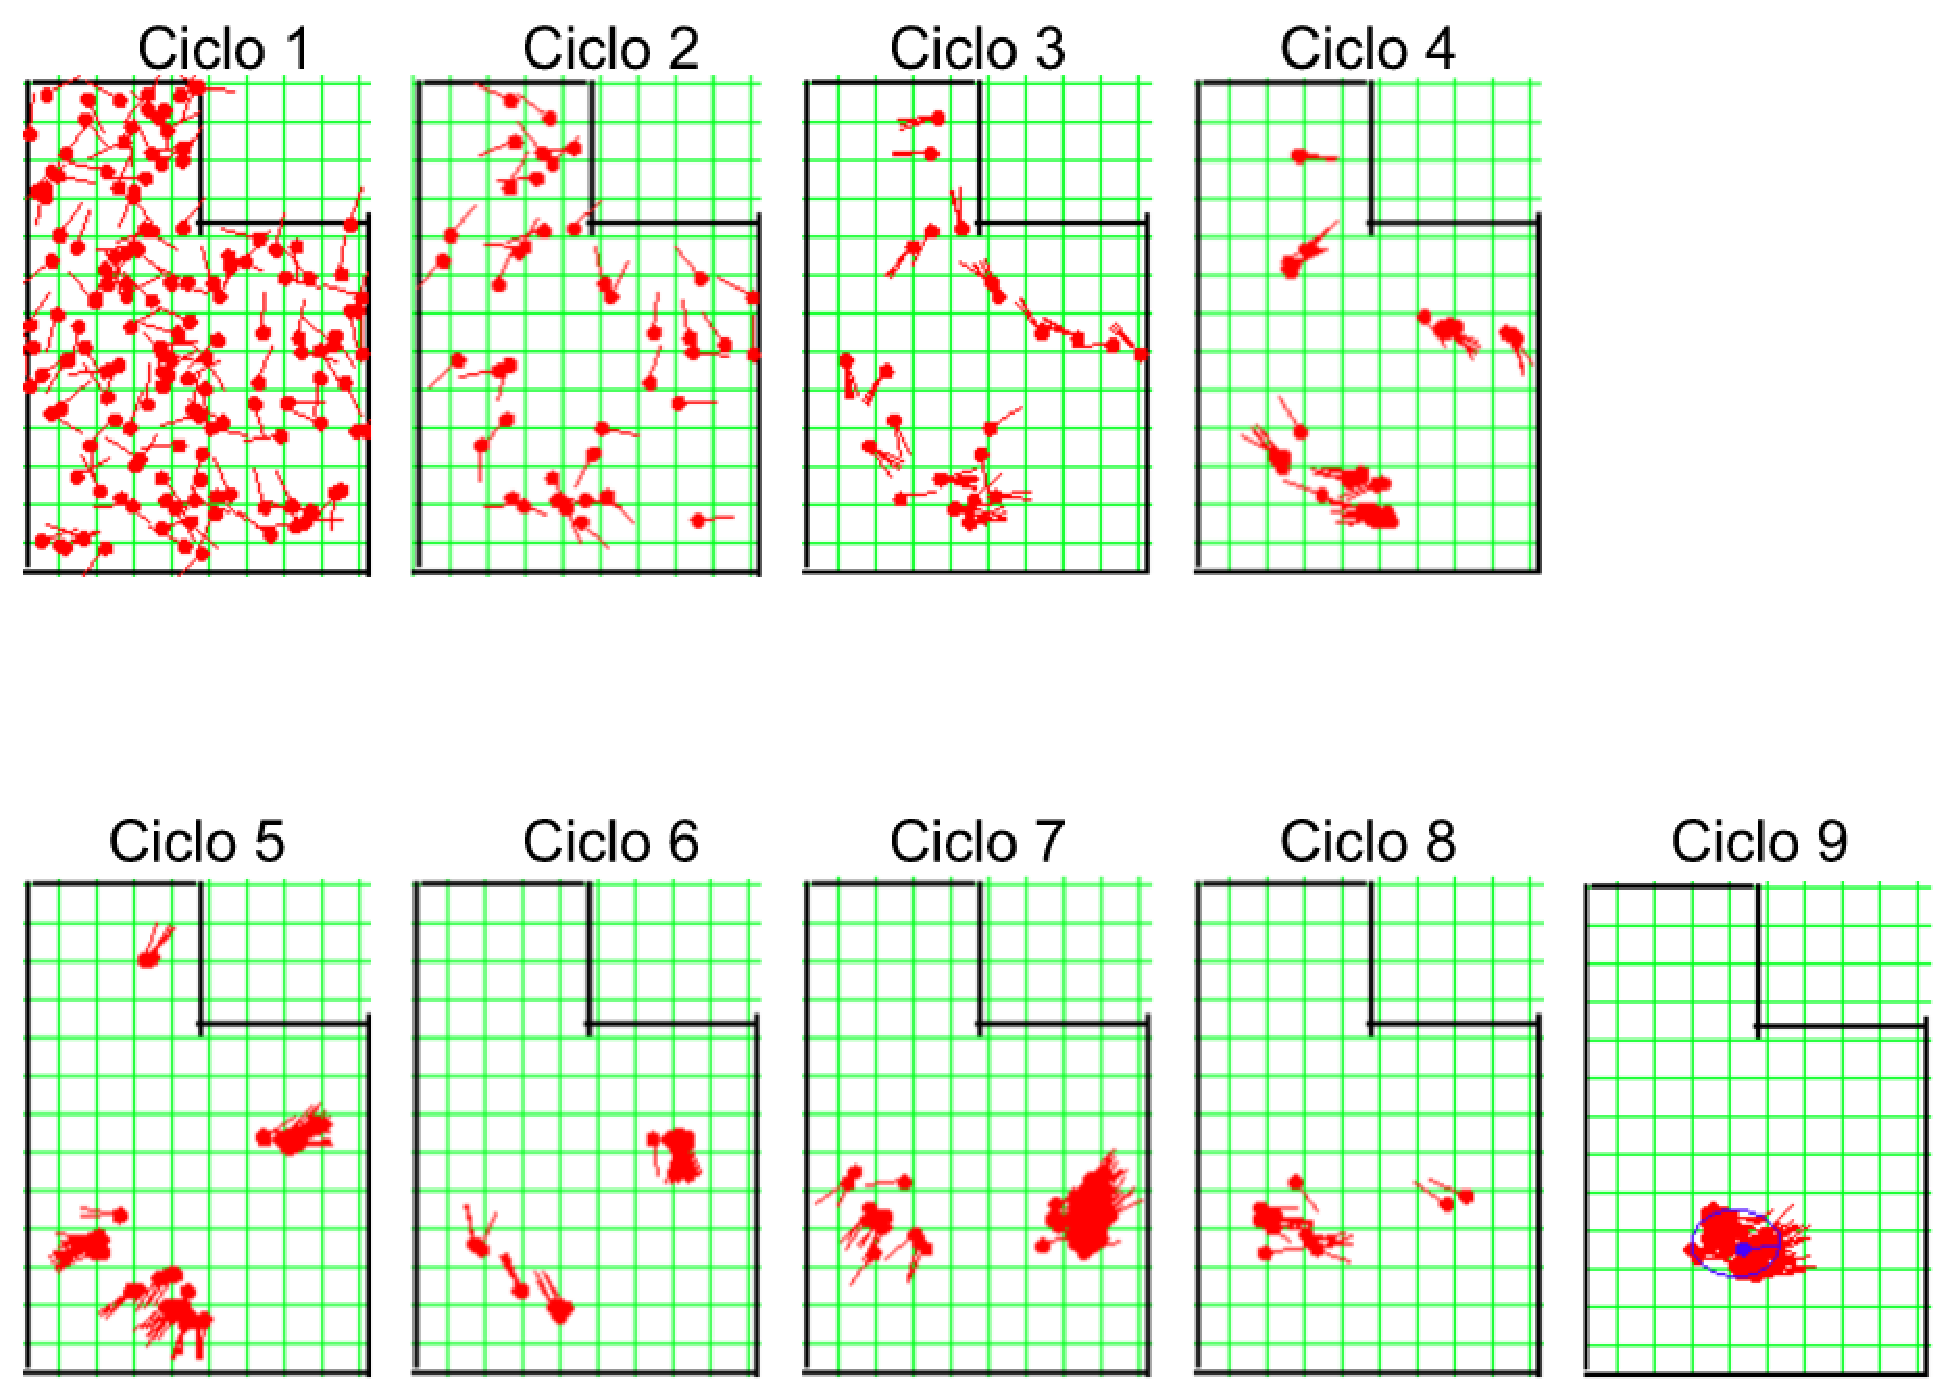
\includegraphics[scale=0.4]{figuras/cen4_ex1.eps}
\captionof{figure}{Caso de Teste 4 - Cenário 1}
\label{img:cen4_ex1}
\par}

{\centering
\includegraphics[scale=0.2]{figuras/real_cen4_ex1.eps}
\captionof{figure}{Posição Real do Caso de Teste 4 - Cenário 1.}
\label{img:real_cen4_ex1}
\par}

\subsection{Cenário 2}

{\centering
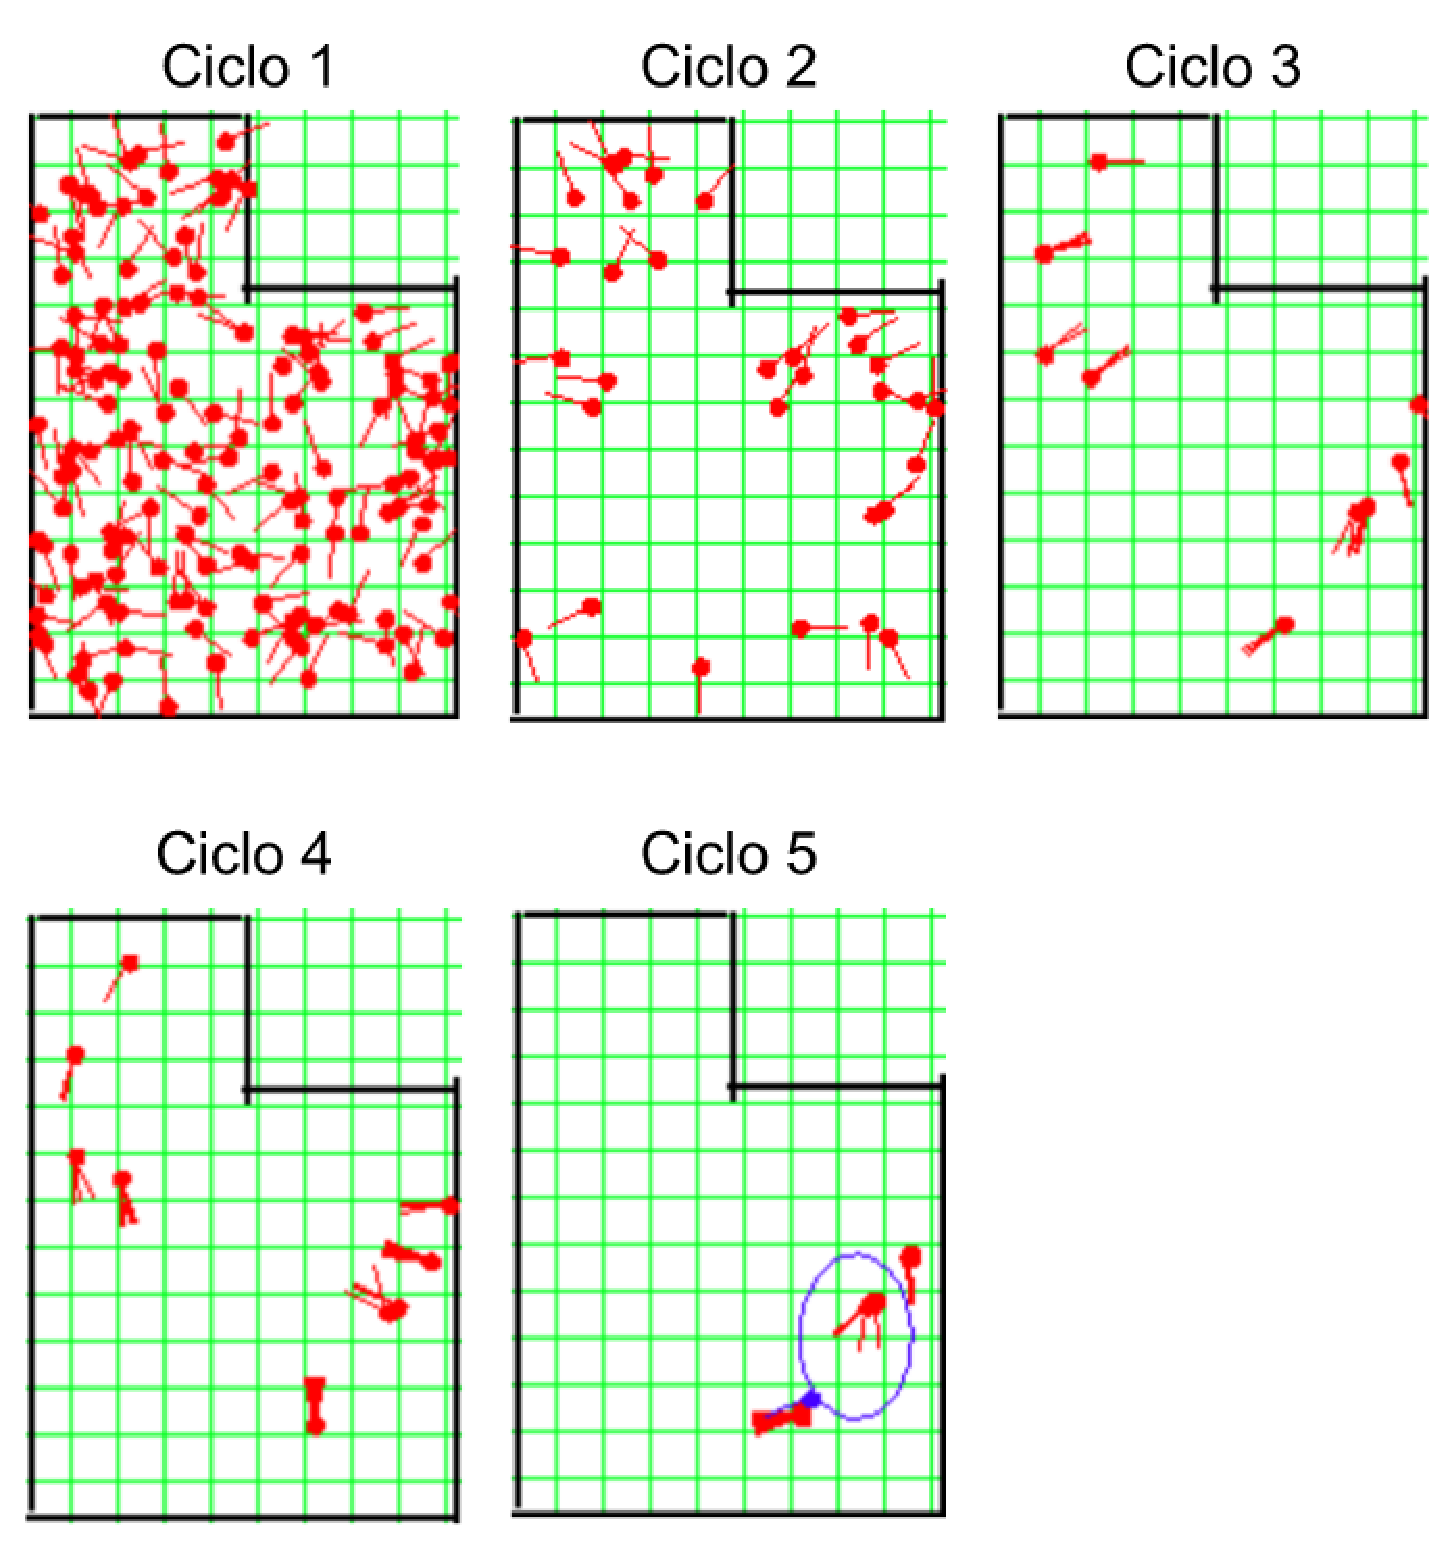
\includegraphics[scale=0.4]{figuras/cen4_ex2.eps}
\captionof{figure}{Caso de Teste 4 - Cenário 2}
\label{img:cen4_ex2}
\par}

{\centering
\includegraphics[scale=0.2]{figuras/real_cen4_ex2.eps}
\captionof{figure}{Posição Real do Caso de Teste 4 - Cenário 2.}
\label{img:real_cen4_ex2}
\par}

\subsection{Cenário 3}

{\centering
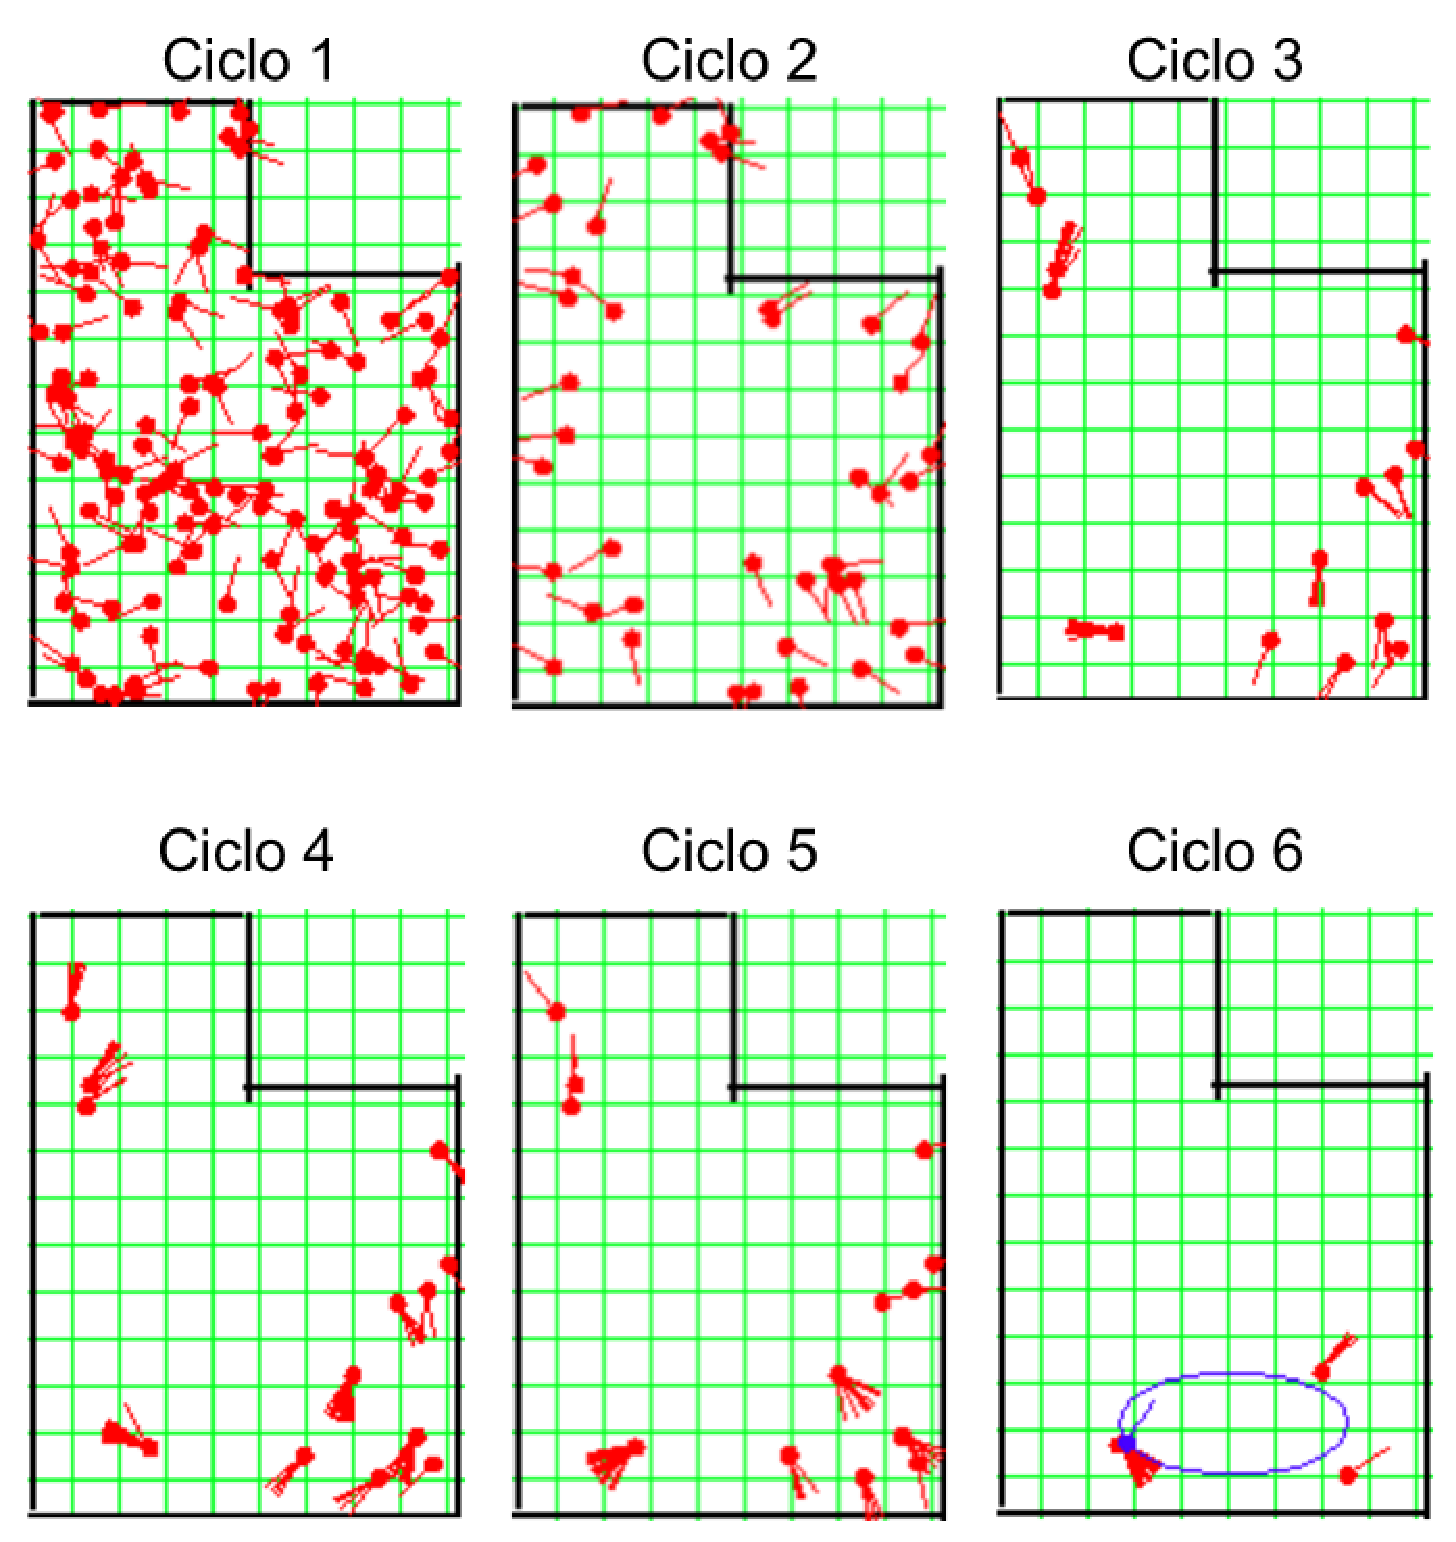
\includegraphics[scale=0.4]{figuras/cen4_ex3.eps}
\captionof{figure}{Caso de Teste 4 - Cenário 3}
\label{img:cen4_ex3}
\par}

{\centering
\includegraphics[scale=0.2]{figuras/real_cen4_ex3.eps}
\captionof{figure}{Posição Real do Caso de Teste 4 - Cenário 3.}
\label{img:real_cen4_ex3}
\par}

\subsection{Cenário 4}

{\centering
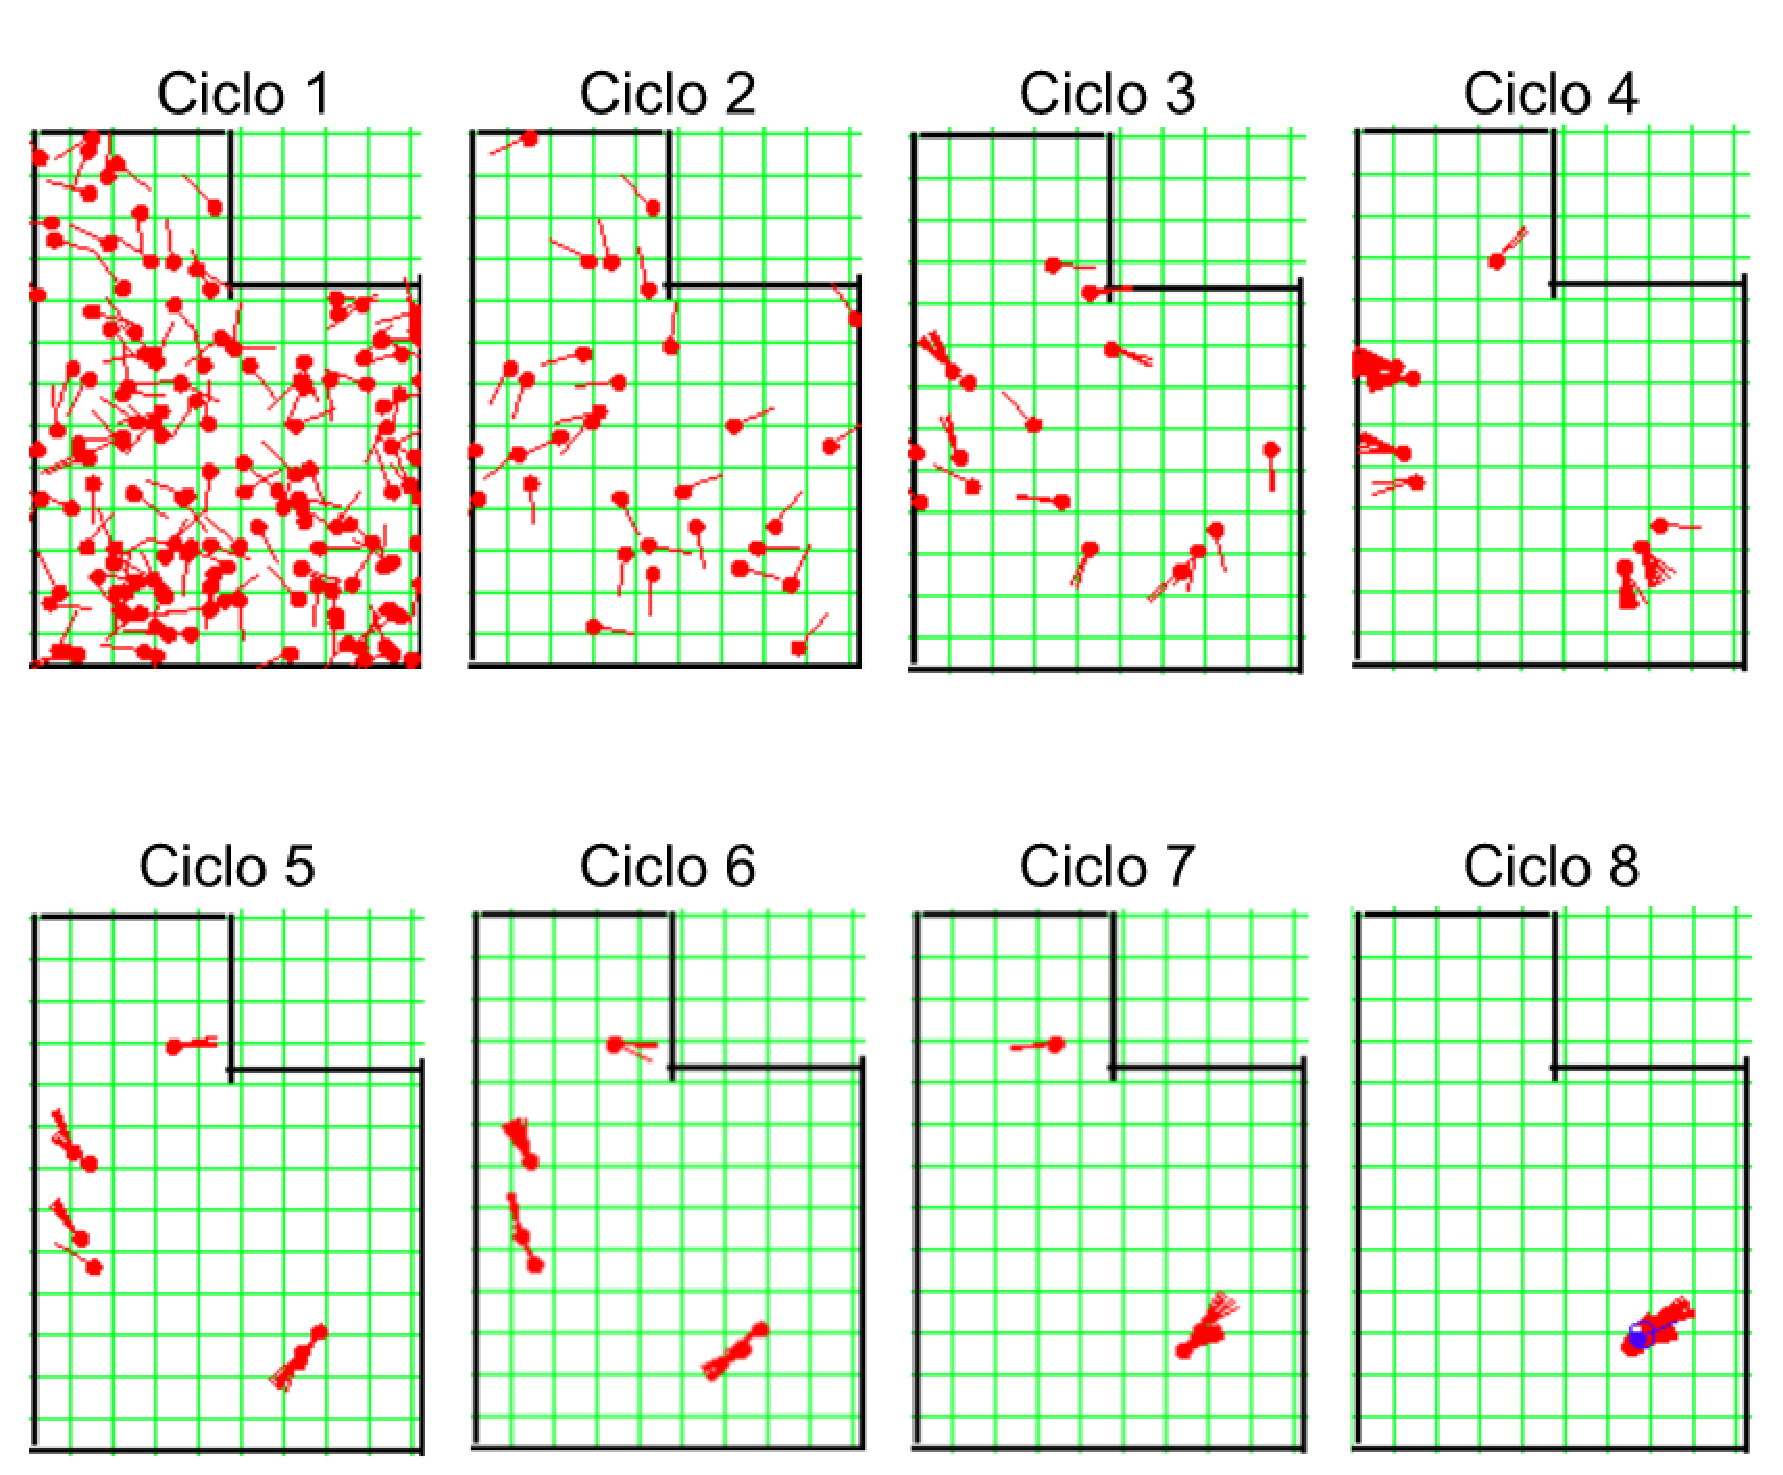
\includegraphics[scale=0.4]{figuras/cen4_ex4.eps}
\captionof{figure}{Caso de Teste 4 - Cenário 4}
\label{img:cen4_ex4}
\par}

{\centering
\includegraphics[scale=0.2]{figuras/real_cen4_ex4.eps}
\captionof{figure}{Posição Real do Caso de Teste 4 - Cenário 4.}
\label{img:real_cen4_ex4}
\par}

\subsection{Cenário 5}

{\centering
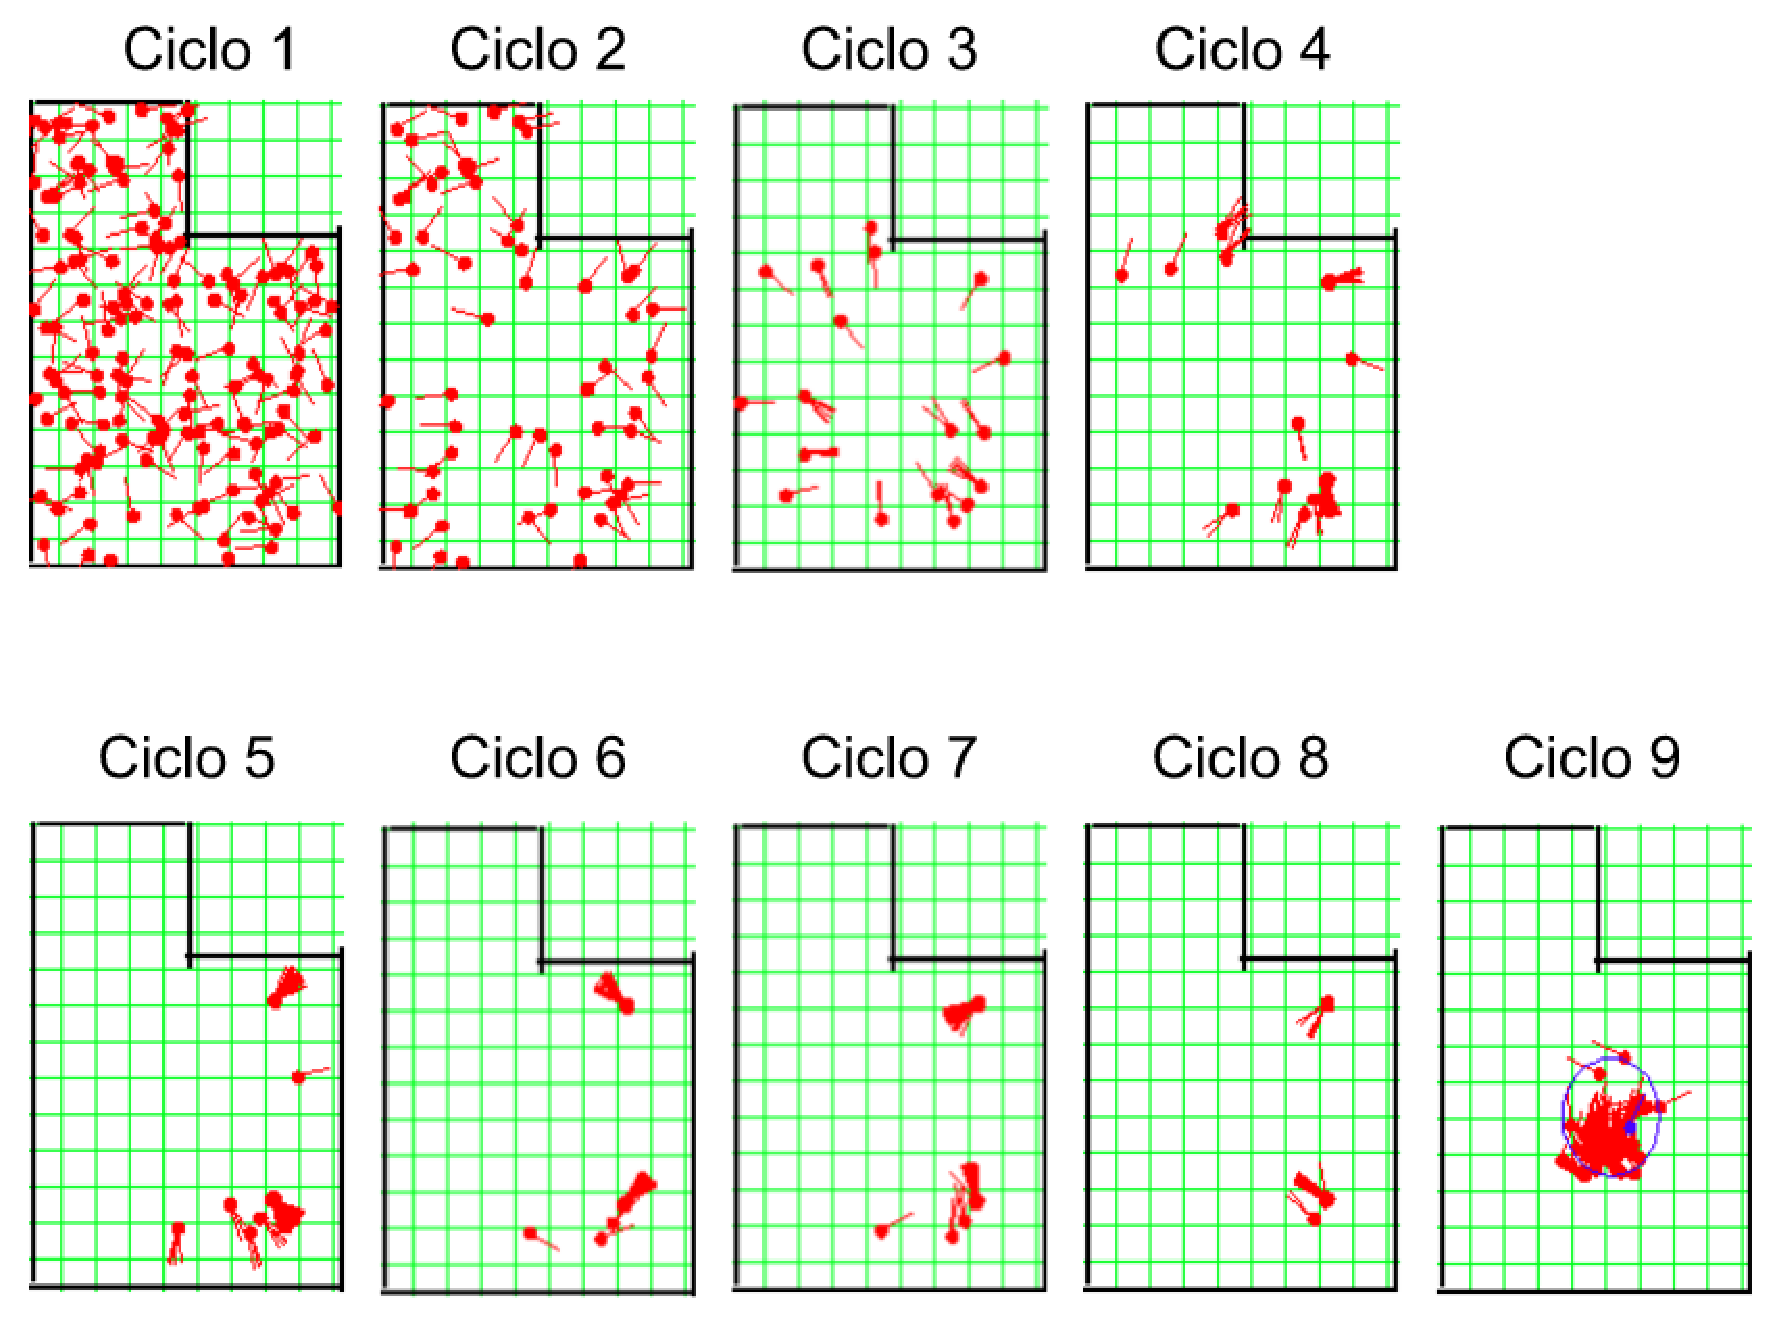
\includegraphics[scale=0.4]{figuras/cen4_ex5.eps}
\captionof{figure}{Caso de Teste 4 - Cenário 5}
\label{img:cen4_ex5}
\par}

{\centering
\includegraphics[scale=0.2]{figuras/real_cen4_ex5.eps}
\captionof{figure}{Posição Real do Caso de Teste 4 - Cenário 5.}
\label{img:real_cen4_ex5}
\par}
